\documentclass[]{article}
\usepackage[T1]{fontenc}
\usepackage{lmodern}
\usepackage{amssymb,amsmath}
\usepackage{ifxetex,ifluatex}
\usepackage{fixltx2e} % provides \textsubscript
% Set line spacing
% use upquote if available, for straight quotes in verbatim environments
\IfFileExists{upquote.sty}{\usepackage{upquote}}{}
\ifnum 0\ifxetex 1\fi\ifluatex 1\fi=0 % if pdftex
  \usepackage[utf8]{inputenc}
\else % if luatex or xelatex
  \ifxetex
    \usepackage{mathspec}
    \usepackage{xltxtra,xunicode}
  \else
    \usepackage{fontspec}
  \fi
  \defaultfontfeatures{Mapping=tex-text,Scale=MatchLowercase}
  \newcommand{\euro}{€}
\fi
% use microtype if available
\IfFileExists{microtype.sty}{\usepackage{microtype}}{}
\usepackage[margin=1in]{geometry}
\ifxetex
  \usepackage[setpagesize=false, % page size defined by xetex
              unicode=false, % unicode breaks when used with xetex
              xetex]{hyperref}
\else
  \usepackage[unicode=true]{hyperref}
\fi
\hypersetup{breaklinks=true,
            bookmarks=true,
            pdfauthor={Yago Durán Cid},
            pdftitle={Applied Logistic Regression - Exercise Week 1},
            colorlinks=true,
            citecolor=blue,
            urlcolor=blue,
            linkcolor=magenta,
            pdfborder={0 0 0}}
\urlstyle{same}  % don't use monospace font for urls
\setlength{\parindent}{0pt}
\setlength{\parskip}{6pt plus 2pt minus 1pt}
\setlength{\emergencystretch}{3em}  % prevent overfull lines
\setcounter{secnumdepth}{0}

%%% Change title format to be more compact
\usepackage{titling}
\setlength{\droptitle}{-2em}
  \title{Applied Logistic Regression - Exercise Week 1}
  \pretitle{\vspace{\droptitle}\centering\huge}
  \posttitle{\par}
  \author{Yago Durán Cid}
  \preauthor{\centering\large\emph}
  \postauthor{\par}
  \predate{\centering\large\emph}
  \postdate{\par}
  \date{16/05/2015}




\begin{document}

\maketitle


\textbf{WEEK 1}

\emph{Exercise 1:}\\Use the Myopia Study (MYOPIA.dta) One variable that
is clearly important is the initial value of spherical equivalent
refraction (SPHEQ).

\begin{enumerate}
\def\labelenumi{\alph{enumi}.}
\itemsep1pt\parskip0pt\parsep0pt
\item
  Write down the equation for the logistic regression model of SPHEQ on
  MYOPIA. Write down the equation for the logit transformation of this
  logistic regression model. What characteristic of the outcome
  variable, MYOPIA, leads us to consider the logistic regression model
  as opposed to the usual linear regression model to describe the
  relationship between MYOPIA and SPHEQ?
\end{enumerate}

Given the data for myopia where y=0 if the subject has myopia and y=1 if
the subject has not got myopia.

To evaluate the probability of a subject has not got myopia given a
value of spherical equivalent refraction x we can write the following
logistic regression model:

$\pi(x)=E(y|x)=\frac{e^{(\beta_0+\beta_1x)}}{1+e^{(\beta_0+\beta_1x)}}$

The odd ratio of the equation above would be:

$Odd\,Ratio=\frac{\pi(x)}{(1-\pi(x))}$

And the natural logarithm of the odd ratio would be:

$ln\bigg(\frac{\pi(x)}{(1-\pi(x))}\bigg)=\beta_0+\beta_1x$

The assumption in the case of a linear regression model is:

$y=E(y|x)+\varepsilon$ where $\varepsilon \rightarrow N(0,\sigma^2)$ and
therefore $y|x~N(E(y|x),\sigma^2)$ which in our case is not true given
that we have only two possible outcomes (1 or 0)

\begin{enumerate}
\def\labelenumi{\alph{enumi}.}
\setcounter{enumi}{1}
\itemsep1pt\parskip0pt\parsep0pt
\item
  Form a scatterplot of MYOPIA vs.~SPHEQ.
\end{enumerate}

\begin{center}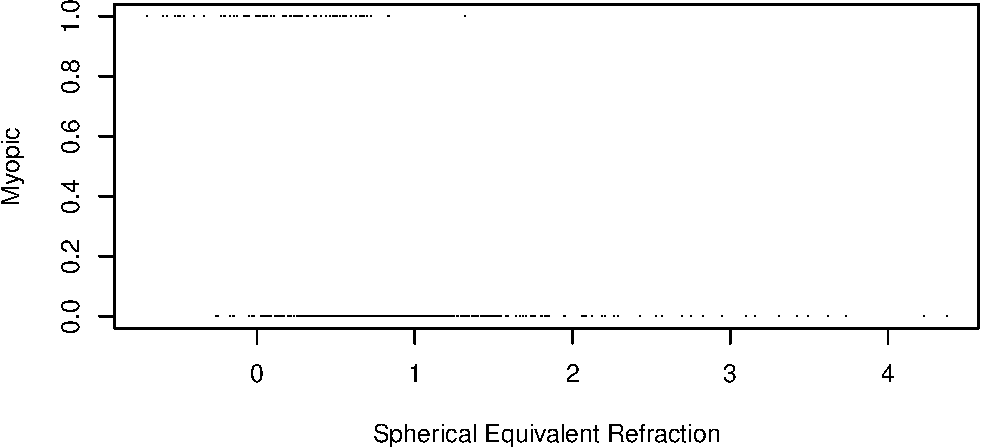
\includegraphics{HomeworkWeek1_files/figure-latex/unnamed-chunk-1-1} \end{center}

\begin{enumerate}
\def\labelenumi{\alph{enumi}.}
\setcounter{enumi}{2}
\itemsep1pt\parskip0pt\parsep0pt
\item
  Write down an expression for the likelihood and log likelihood for the
  logistic regression model in part (a) using the ungrouped, n = 618 ,
  data. Obtain expressions for the two likelihood equations.
\end{enumerate}

$\ell(\beta)=\prod_{i=1}^{n}[\pi(x_i)]^{y_i}[1-\pi(x_i)]^{1-y_i}$

applying natural logarithm to expression above

$L(\beta)=ln(\ell(\beta))=\sum_{i=1}^{n}y_iln[\pi(x_i)]+(1-y_i)ln[1-\pi(x_i)]$

The likelihood equations are:

$\sum_{i=1}^{n}(y_i-\pi(x_i))=0$ $\sum_{i=1}^{n}x_i(y_i-\pi(x_i))=0$

\begin{enumerate}
\def\labelenumi{\alph{enumi}.}
\setcounter{enumi}{3}
\itemsep1pt\parskip0pt\parsep0pt
\item
  Obtain the maximum likelihood estimates of the parameters of the
  logistic regression model in part (a). These estimates should be based
  on the ungrouped, n = 618 ,data. Using these estimates, write down the
  equation for the fitted values, that is, the estimated logistic
  probabilities. Plot the equation for the fitted values on the axes
  used in the scatterplots in parts (b) and (c).
\end{enumerate}

\begin{verbatim}
## 
## Call:
## glm(formula = MYOPIC ~ SPHEQ, family = "binomial", data = data)
## 
## Deviance Residuals: 
##     Min       1Q   Median       3Q      Max  
## -1.6435  -0.4533  -0.2681  -0.1029   3.1602  
## 
## Coefficients:
##             Estimate Std. Error z value Pr(>|z|)    
## (Intercept)  0.05397    0.20675   0.261    0.794    
## SPHEQ       -3.83310    0.41837  -9.162   <2e-16 ***
## ---
## Signif. codes:  0 '***' 0.001 '**' 0.01 '*' 0.05 '.' 0.1 ' ' 1
## 
## (Dispersion parameter for binomial family taken to be 1)
## 
##     Null deviance: 480.08  on 617  degrees of freedom
## Residual deviance: 337.34  on 616  degrees of freedom
## AIC: 341.34
## 
## Number of Fisher Scoring iterations: 6
\end{verbatim}

Substituting with the estimated values we get:

$\pi_{e}(x)=\frac{e^{(0.05397-3.8331x)}}{(1+e^{(0.05397-3.8331x)})}$

\begin{center}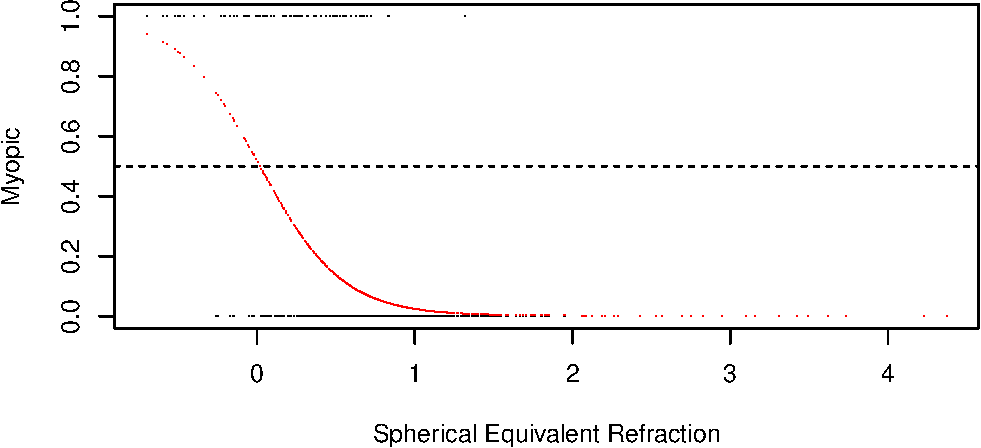
\includegraphics{HomeworkWeek1_files/figure-latex/unnamed-chunk-3-1} \end{center}

\emph{Exercise 2:}\\Use the ICU study (icu.dta) The ICU data set
consists of a sample of 200 subjects who were part of a much larger
study on survival of patients following admission to an adult intensive
care unit (ICU). The major goal of this study was to develop a logistic
regression model to predict the probability of survival to hospital
discharge of these patients. A number of publications have appeared
which have focused on various facets of this problem.

\begin{enumerate}
\def\labelenumi{\alph{enumi}.}
\itemsep1pt\parskip0pt\parsep0pt
\item
  Write down the equation for the logistic regression model of STA on
  AGE. Write down the equation for the logit transformation of this
  logistic regression model. What characteristic of the outcome
  variable, STA, leads us to consider the logistic regression model as
  opposed to the usual linear regression model to describe the
  relationship between STA and AGE?
\end{enumerate}

The logistic regression model is:

$\pi(x)=E(y|x)=\frac{e^{(\beta_0+\beta_1x)}}{1+e^{(\beta_0+\beta_1x)}}$
$where\,x=AGE\,and\,\pi(x)= Prob(STA=1|AGE)$

Being the logit transformation:

$ln\bigg(\frac{\pi(x)}{(1-\pi(x))}\bigg)=\beta_0+\beta_1x$

Usual linear regression analysis is not recommended given the binary
nature of STA

\begin{enumerate}
\def\labelenumi{\alph{enumi}.}
\setcounter{enumi}{1}
\itemsep1pt\parskip0pt\parsep0pt
\item
  Form a scatterplot of STA versus AGE.c. Write down an expression for
  the likelihood and log likelihood for the logistic regression model in
  part (a) using the ungrouped, n = 200 , data. Obtain expressions for
  the two likelihood equations.
\end{enumerate}

\begin{center}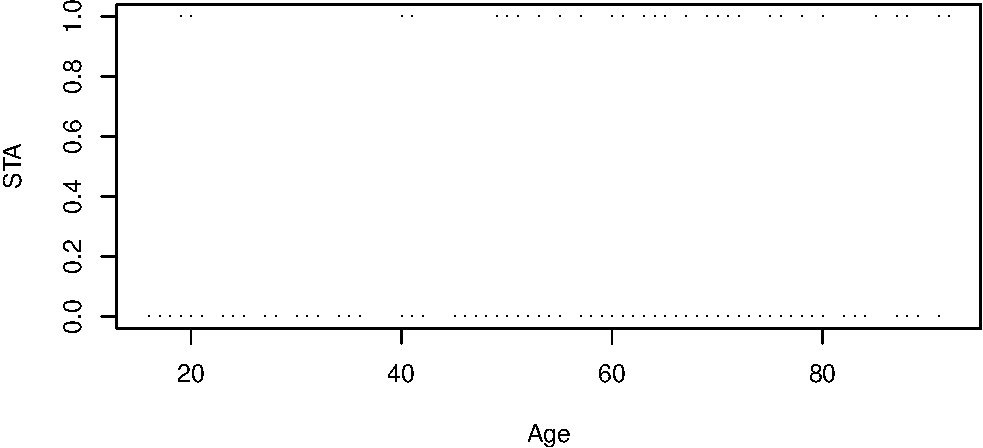
\includegraphics{HomeworkWeek1_files/figure-latex/unnamed-chunk-4-1} \end{center}

$\ell(\beta)=\prod_{i=1}^{n}[\pi(x_i)]^{y_i}[1-\pi(x_i)]^{1-y_i}$\\$where\,x=AGE\,and\,y_i=0\,if\,the\,patient\,lived\,or\,y_i=1\,if\,the\,patient\,died$

applying natural logarithm to expression above

$L(\beta)=ln(\ell(\beta))=\sum_{i=1}^{n}y_iln[\pi(x_i)]+(1-y_i)ln[1-\pi(x_i)]$

The likelihood equations are:

$\sum_{i=1}^{n}(y_i-\pi(x_i))=0$ $\sum_{i=1}^{n}x_i(y_i-\pi(x_i))=0$

\begin{enumerate}
\def\labelenumi{\alph{enumi}.}
\setcounter{enumi}{3}
\itemsep1pt\parskip0pt\parsep0pt
\item
  Obtain the maximum likelihood estimates of the parameters of the
  logistic regression model in part (a). These estimates should be based
  on the ungrouped, n = 200 , data. Using these estimates, write down
  the equation for the fitted values, that is, the estimated logistic
  probabilities. Plot the equation for the fitted values on the axes
  used in the scatterplots in part (b).
\end{enumerate}

\begin{verbatim}
## 
## Call:
## glm(formula = STA ~ AGE, family = "binomial", data = icu)
## 
## Deviance Residuals: 
##     Min       1Q   Median       3Q      Max  
## -0.9536  -0.7391  -0.6145  -0.3905   2.2854  
## 
## Coefficients:
##             Estimate Std. Error z value Pr(>|z|)    
## (Intercept) -3.05851    0.69608  -4.394 1.11e-05 ***
## AGE          0.02754    0.01056   2.607  0.00913 ** 
## ---
## Signif. codes:  0 '***' 0.001 '**' 0.01 '*' 0.05 '.' 0.1 ' ' 1
## 
## (Dispersion parameter for binomial family taken to be 1)
## 
##     Null deviance: 200.16  on 199  degrees of freedom
## Residual deviance: 192.31  on 198  degrees of freedom
## AIC: 196.31
## 
## Number of Fisher Scoring iterations: 4
\end{verbatim}

Substituting with the estimated values we get:

$\pi_{e}(x)=\frac{e^{(-3.05851+0.02754AGE)}}{(1+e^{(-3.05851-0.02754AGE)})}$

And the logit transformation:

$g(x)=-3.05851-0.02754AGE$

\begin{center}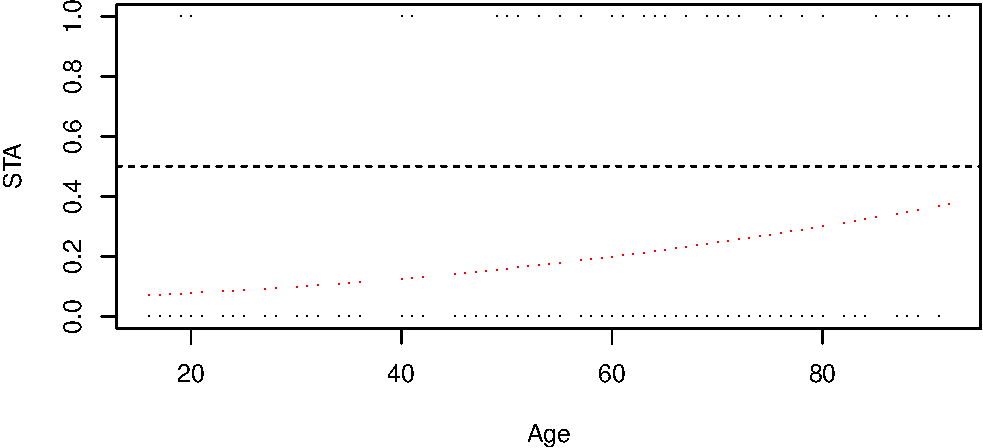
\includegraphics{HomeworkWeek1_files/figure-latex/unnamed-chunk-6-1} \end{center}

\begin{enumerate}
\def\labelenumi{\alph{enumi}.}
\setcounter{enumi}{4}
\itemsep1pt\parskip0pt\parsep0pt
\item
  Summarize (describe in words) the results presented in the plot
  obtained from parts (b) and (d).
\end{enumerate}

Given the dichotomous nature of the STA variable (patients or live or
die) Logistic Regression is appropriate to understand the impact of age
on the probability of surviving hospital discharge.\\From estimated
parameters it seems that as the age increases the probability of survive
to hospital discharge reduces.

\end{document}
